In this section, we analyze the impact of uniform quantization on the generalization performance of linear regression models trained on top of the word embeddings.
We present two results:
First, we show that when the embedding matrix is quantized to $b$ bits, and the linear ridge regression model is trained with regularization parameter $\lambda$, we attain good generalization bounds for the quantized features relative to the full-precision features when $2^b \lambda$ is large.
Second, we show that if the singular values of the embedding matrix decay slowly, then training the regression model with a large regularization parameter $\lambda$ cannot perform much worse than training with a smaller one.
Combining this theoretical result with our empirical observation that the singular values of embedding matrices typically decay slowly provides a principled explanation for why low-precision embeddings perform well on various tasks.

We begin, however, by reviewing generalization bounds for fixed design linear ridge regression.

\subsection{Background: Generalized Bounds for Fixed Design Linear Ridge Regression}
In fixed design linear regression, one is given a dataset $\{(x_i,y_i)\}_{i=1}^n$, for $x_i \in \RR^d$ and $y_i = \by_i + \eps_i \in \RR$, where the $\eps_i$ are independent random perturbations of the ``true labels'' $\by_i$ satisfying $\expect{}{\eps_i} = 0$ and $\var{}{\eps_i} = \sigma^2 < \infty$.
The goal is to design a training algorithm which takes as input the noisy dataset $\{(x_i,y_i)\}_{i=1}^n$ and outputs a model $f(x) = w^T x$ for which $\expect{}{\frac{1}{n}\sum_i (f(x_i) -\by_i)^2} \eqdef \cR(f)$ is small.
Linear ridge regression selects $w^* = \argmin_w \sum_i (w^T x_i - y_i)^2 + \lambda\|w\|_2^2$.
Letting $X \in \RR^{n\times d}$ be the matrix whose rows are $x_i$, $y \defeq (y_1,...,y_n) \in \RR^d$, and $I_d$ be the $d$-dimensional identity matrix, the minimizer of this optimization problem is $w^* = ( X^T X + \lambda I_d)^{-1}X^Ty$.
It is easy to show \citep{alaoui15} that the expected generalization error for the model $f_X(x) \defeq w^{*T}x$ is
\begin{eqnarray*}
\cR(f_X) &=& \frac{\lambda^2}{n} \by^T(XX^T + \lambda I_n)^{-2}\by \; +\\ && \frac{\sigma^2}{n}\tr\Big((XX^T)^2(XX^T + \lambda I_n)^{-2}\Big).
\end{eqnarray*}

The question we ask in this work is: when we replace $X$ by an approximation $\tX$, how close will $\cR(f_{\tX})$ be to $\cR(f_X)$?
To answer this question, we intuitively require two things: a notion of distance between $X$ and $\tX$, and an upper bound for $\cR(f_{\tX})$ in terms of $\cR(f_X)$ and the distance between $X$ and $\tX$.
For both of these components, we leverage the recent work of \citep{lprff18}.
In that work, they define the following notion of distance between two matrices:

\begin{definition}{\citep{lprff18}}
	\label{def:specdist}
	For $\Delta_1, \Delta_2 \geq 0$, a symmetric matrix $A$ is a \emph{$(\Delta_1, \Delta_2)$-spectral approximation} of another symmetric matrix $B$ if $(1-\Delta_1)B \preceq A \preceq (1+\Delta_2)B$. 
\end{definition}

By applying this definition to $\tX\tX^T + \lambda I_n$ and $XX^T + \lambda I_n$, the authors prove the following generalization bound:
\begin{proposition}{(Adapted from \citep{lprff18})}
	Let $K \defeq XX^T$ and $\tK \defeq \tX\tX^T$, and suppose $\tK + \lambda I_n$ is $(\Delta_1, \Delta_2)$-spectral approximation of $K+\lambda I_n$, for $\Delta_1 \in [0,1)$, $\Delta_2 \geq 0$.
	Let $d$ denote the rank of $\tX$, and let $f_{X}$ and $f_{\tX}$ be the ridge regression estimators learned using these matrices, with regularizing constant $\lambda \geq 0$ and label noise variance $\sigma^2 < \infty$. Then
	\begin{equation}
	\cR(f_{\tX}) \leq \frac{1}{1-\Delta_1} \hcR(f_X) +  \frac{\Delta_2}{1+\Delta_2}\frac{d}{n}\sigma^2,
	\label{eq:risk_bound}
	\end{equation}
	where 
	\begin{eqnarray*}
	\hcR(f_X) &\defeq& \frac{\lambda}{n} \by^T(K+\lambda I)^{-1}\by + \frac{\sigma^2}{n}\tr\Big(K(K+\lambda I)^{-1}\Big) \\
	&\geq& \cR(f_X).
%	\label{eq:avron_rhat}
	\end{eqnarray*}
	\label{prop:genbound}
\end{proposition}
\todo{Discuss how what we will show differs from what is shown in kernel paper.}

\subsection{Theoretical Results}
We now show that our compression algorithm with high probability produces an embedding matrix which is a close spectral approximation of the full-precision matrix, in terms of $(\Delta_1,\Delta_2)$.
Combining this with the Proposition~\ref{prop:genbound} yields a generalization bound for the compressed embeddings.
A consequence of our bound is that when the regularization parameter is large, lower precision can be used for the embeddings without affecting $\Delta_1$ and $\Delta_2$.
We show that in the case of word embeddings with slowly-decaying singular values, a large regularization parameter $\lambda$ (and thus, a low-precision $b$) can be used without significantly affecting generalization performance.
Our empirical observation that embedding matrices have slowly decaying singular values thus helps explain why our compression algorithm is able to attain strong generalization performance at very low levels of precision.

We now present our main theoretical result, deferring all proofs to the Appendix:
\begin{theorem}
	\label{thm:main}
	Let $X \in \RR^{n\times d}$ be an embedding matrix with corresponding Gram matrix $K \defeq XX^T$, where we assume all entries $X_{ij} \in [-\frac{1}{\sqrt{d}},\frac{1}{\sqrt{d}}]$; let $\tX\defeq X+C$ denote a $b$-bit quantization of $X$, with $\tK \defeq \tX\tX^T$ the kernel matrix of the quantized data matrix. Here, $C$ denotes the quantization noise, with $\expect{}{C_{ij}} = 0$ and $\var{}{C_{ij}} \leq \delta_b^2/d \;\;\forall i,j$, where $\delta_b^2 \defeq (2^b-1)^{-2}$, and $b$ is the number of bits used per feature.
	Then for any $\Delta_1 \geq 0, \Delta_2 \geq \delta^2_b/\lambda$,
	\begin{eqnarray*}
	&&\hspace{-0.37in}\Prob\Big[(1- \Delta_1) (K + \lambda I_n) \preceq \tK + \lambda I_n \preceq (1 + \Delta_2) (K + \lambda I_n)
	\Big] 
	\\ &\geq& 1 - 
	n \exp \bigg(\frac{-\Delta_1^2}{2dL^2 + (2L/3)\Delta_1}\bigg) \\
	&&- n \exp \bigg(\frac{-(\Delta_2-\delta_b^2/\lambda)^2}{2dL^2 + (2L/3)(\Delta_2-\delta_b^2/\lambda)}\bigg),
	\end{eqnarray*}
	for $L \defeq 5 \cdot \frac{2^b \cdot \delta_b^2}{\lambda}\cdot \frac{n}{d}$.
\end{theorem}
Note that in this theorem, we assume the embedding matrix is bounded, whereas in the actual implementation of our compression algorithm (Alg.~\ref{alg:smallfry}) we enforce this constraint artificially by searching for the optimal threshold at which to clip the matrix entries.
To better understand the implications of the above theorem, we present the following corollary:
\begin{corollary}
	\label{cor:main}
	If $\Delta_1 \geq \frac{\log(n/\rho)L}{3}\Big(1+\sqrt{1+\frac{18d}{\log(n/\rho)}}\Big) \approx \frac{5n}{2^b \lambda}\sqrt{\frac{2\log(n/\rho)}{d}}$,
	then $\Prob\big[(1 - \Delta_1) (K + \lambda I_n) \preceq \tK + \lambda I_n \big] \geq  1 - \rho$. 
	Similarly, if $\Delta_2 \geq \frac{\delta_b^2}{\lambda} +  \frac{\log(n/\rho)L}{3}\Big(1+\sqrt{1+\frac{18d}{\log(n/\rho)}}\Big) \approx \frac{1}{2^{2b}\lambda} + \frac{5n}{2^b \lambda}\sqrt{\frac{2\log(n/\rho)}{d}}$,
	then $\Prob\big[\tK + \lambda I_n \preceq (1 + \Delta_2) (K + \lambda I_n)\big] \geq  1 - \rho$. 
\end{corollary}

This corollary makes clear that if $2^b\lambda$ is large, the $b$-bit compressed embedding matrix will be a close spectral approximation of the full-precision matrix, for small $\Delta_1$ and $\Delta_2$.
In the following theorem, we show that when the smallest singular value of $X^TX$ is large, using a large regularization parameter $\lambda$ will not significantly harm the generalization performance of $f_X$, relative to using a smaller $\lambda$.
Combining this result with Proposition~\ref{prop:genbound} and Theorem~\ref{thm:main}, we can conclude that the generalization performance of a linear model trained on low-precision features with a large regularizer $\lambda$ will not be much worse than the performance of a model trained on the full-precision features with any $\lambda' \leq \lambda$.
We now present the result:

\begin{theorem}
	\label{thm:large_lambda}
	Let $X$ be an embedding matrix, and $\by$ be the corresponding vector of labels. Let $\sm$ be the smallest eigenvalue of $X^T X$, and let $\lambda_1, \lambda_2$ be two scalars such that $0 \leq \lambda_1 \leq \lambda_2 \leq a\cdot \sm$, for some $a \in [0,1]$. Letting $\cR_{\lambda}(K)$ denote the expected loss when training with regularizer $\lambda$, Gram matrix $K = XX^T$, and label noise $\sigma^2$, we get that:
	\begin{equation}
	R_{\lambda_2}(XX^T) - R_{\lambda_1}(XX^T) \leq a^2\|y\|^2/n
	\label{eq1}
	\end{equation}
\end{theorem}
Intuitively, this theorem shows that if there are no directions in the input space with very small variance, then using a large regularizer will not hurt performance significantly relative to using a smaller regularizer.
This makes sense because the directions of small variance are the ones which are effectively ignored when strong regularization is used.
For the purposes of this work, this theorem shows that if the embedding matrix has a large smallest eigenvalue, it should be possible to attain strong generalization performance with low-precision and a large regularizer.
In practice, we observe that it is common for embedding matrices to have slowly decaying spectra, and thus have a large smallest eigenvalue;
we present plots of the singular values for fastText and Glove embeddings in Figure~\ref{fig:real_spectra}.

\subsection{Empirical Validation of Theory}
In this section, we empirically validate two important predictions made by the above theoretical results:
\begin{enumerate}
	\item When $2^b \lambda$ is large, $\Delta_1$ and $\Delta_2$ are small (Figure~\ref{fig:micro_d1d2}).
	\item When $X^T X$ has a large smallest eigenvalue, generalization performance is not significantly harmed by using a large regularizer
	(Figure~\ref{fig:micro_large_sigma_min}).
\end{enumerate}

In addition, we show that in general word embedding matrices have a relatively large smallest singular value (Figure~\ref{fig:real_spectra}).

\begin{figure*}
	\centering
	\begin{tabular}{c c}
		%		\begin{tabular}{@{\hskip -0.0in}c@{\hskip -0.0in}c@{\hskip -0.0in}c@{\hskip -0.0in}}
		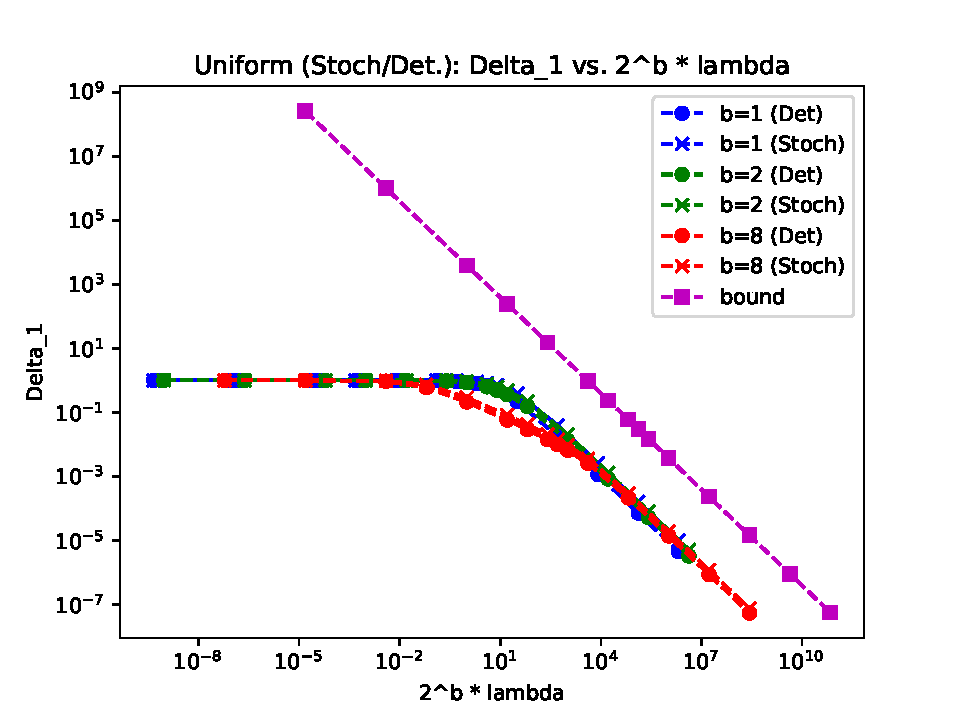
\includegraphics[width=0.4\linewidth]{figures/micro_uniform_nonadapt_delta1_vs_2_b_lambda.pdf} &	
		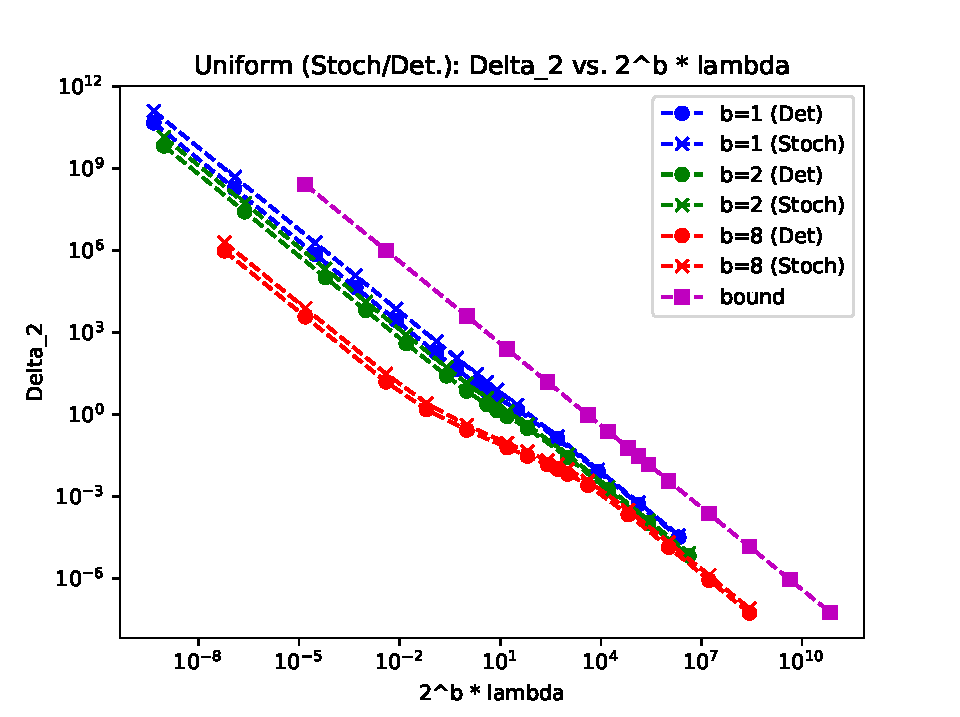
\includegraphics[width=0.4\linewidth]{figures/micro_uniform_nonadapt_delta2_vs_2_b_lambda.pdf}
	\end{tabular}
	\caption{We plot $\Delta_1$ (left) and $\Delta_2$ (right) as a function of $2^b\lambda$, on a randomly generated matrix $X\in\RR^{1000\times 30}$ ($X_{ij}\sim U([-\frac{1}{\sqrt{30}},\frac{1}{\sqrt{30}}])$), for various precisions $b$ and $\lambda$ values.  We show that $2^b \lambda$ largely determines the values of $\Delta_1$ and $\Delta_2$ after compression, as predicted by our theoretical results. We plot results for both deterministic quantization and stochastic quantization, and see that they perform quite similarly by these metrics (though deterministic does perform slightly better on $\Delta_2$). We additionally plot the bounds for $\Delta_1$ and $\Delta_2$ from Corollary~\ref{cor:main}, and see that while the bounds are not tight, their trajectory is matched by the real data.}
	\label{fig:micro_d1d2}
\end{figure*}

\begin{figure}
	\begin{center}
		\centerline{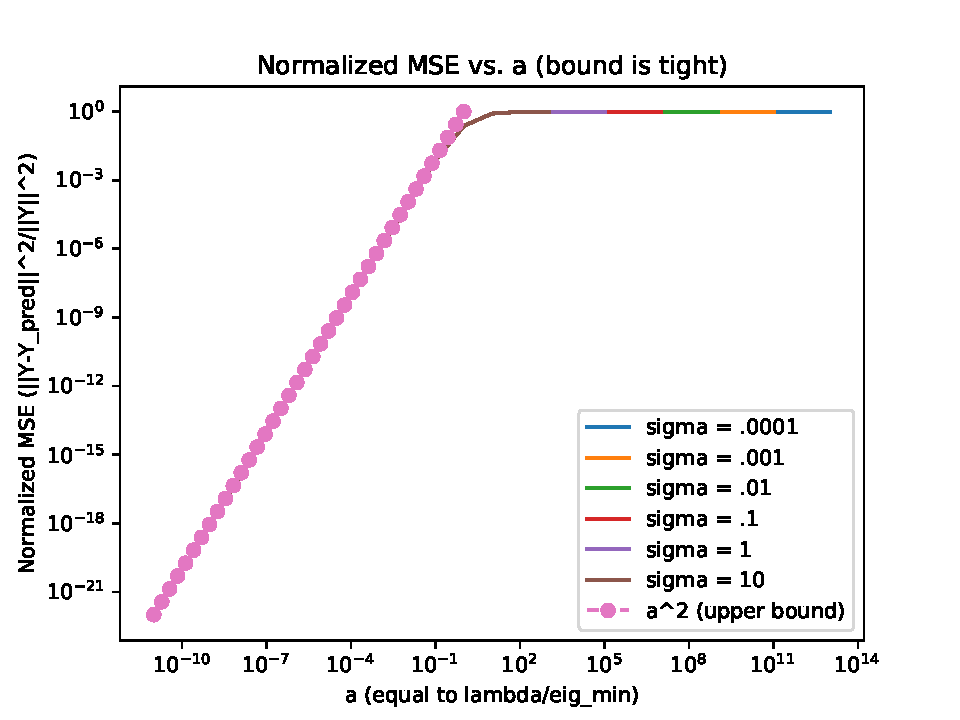
\includegraphics[width=0.8\columnwidth]{figures/micro_large_sigma_min.pdf}}
		\caption{We show that the ratio $a=\frac{\lambda}{\sigma_{min}}$ between the regularization parameter $\lambda$ and the smallest eigenvalue $\sigma_{min}$ of $X^T X$ is very predictive of the degradation in generalization performance $\|\by - y_{pred}\|^2/\|\by\|^2$, as predicted by Theorem~\ref{thm:large_lambda}.
		In particular, we generate an i.i.d. Gaussian matrix $X\in \RR^{1000\times 2}$ for various standard deviations $\sigma$, and consider the noiseless model $\by_i = [0,1]^T x_i$.
		We then solve for the optimal ridge regression model for various values of $\lambda$, and plot $a$ vs.\ the normalized degradation in generalization performance of this model. \todo{TODO: Perhaps plot a more realistic example?}
		}
		\label{fig:micro_large_sigma_min}
	\end{center}
\end{figure}

\begin{figure*}
	\centering
	\begin{tabular}{c c}
		%		\begin{tabular}{@{\hskip -0.0in}c@{\hskip -0.0in}c@{\hskip -0.0in}c@{\hskip -0.0in}}
		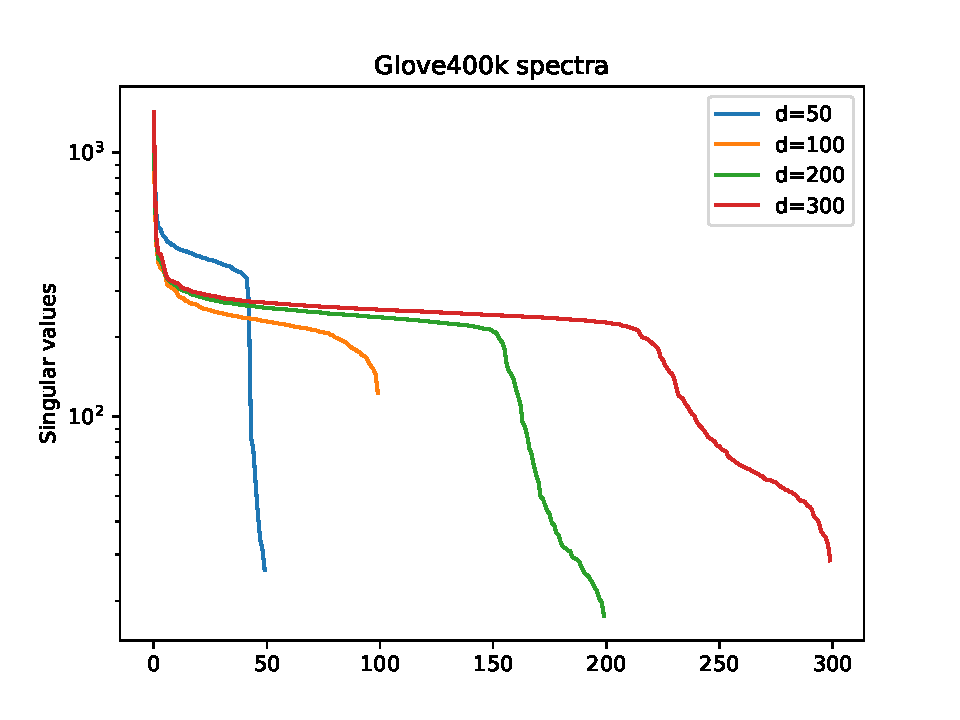
\includegraphics[width=0.4\linewidth]{figures/glove400k_spectra.pdf} &	
		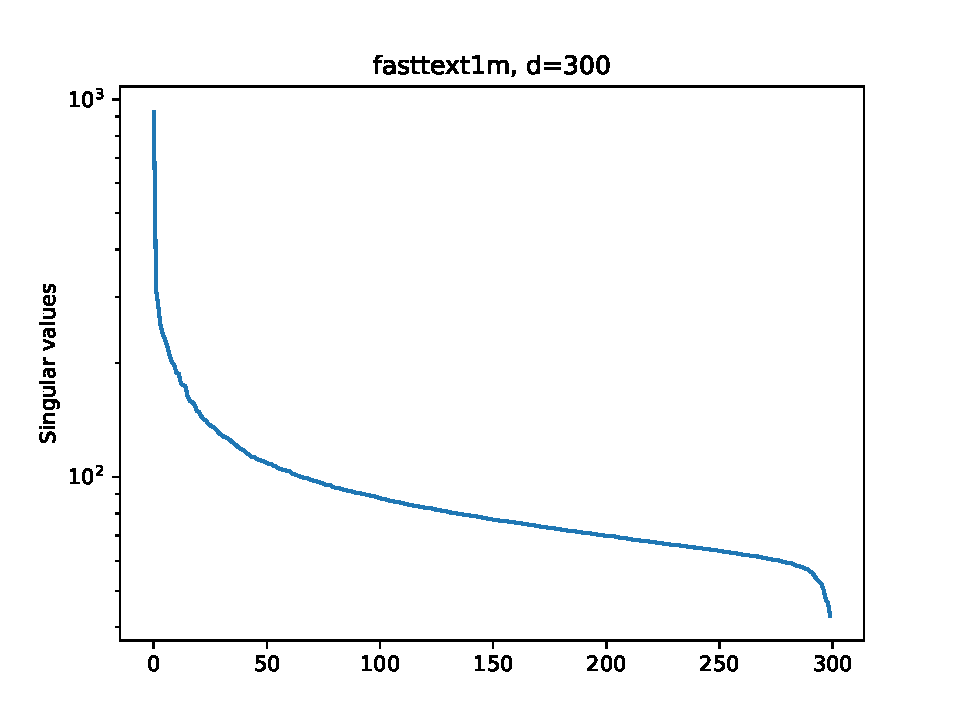
\includegraphics[width=0.4\linewidth]{figures/fasttext1m_spectra.pdf}
	\end{tabular}
	\caption{We plot the real spectra of the pre-trained GloVe ($d \in \{50,100,200,300\}$) and fastText ($d=300$) embedding matrices.
	The smallest singular values are generally only 1 or 2 orders of magnitude smaller than the largest.}
	\label{fig:real_spectra}
\end{figure*}

\subsection{Effect of Clipping on $(\Delta_1,\Delta_2)$}
One way to understand why it is important for us to search for the optimal clipping value in Algorithm~\ref{alg:smallfry} is by understanding the way clipping and quantization together impact $\Delta_1$ and $\Delta_2$.
This perspective reveals that there is a fundamental trade-off between $\Delta_1$ and $\Delta_2$ when choosing the clipping value:
if the clip value is too large, then $\Delta_2$ becomes very large, while if the clip value is too small, then $\Delta_1$ becomes very large.
We demonstrate this in Figure~\ref{fig:deltas_vs_clip_quant}
\begin{figure}
	\begin{center}
		\centerline{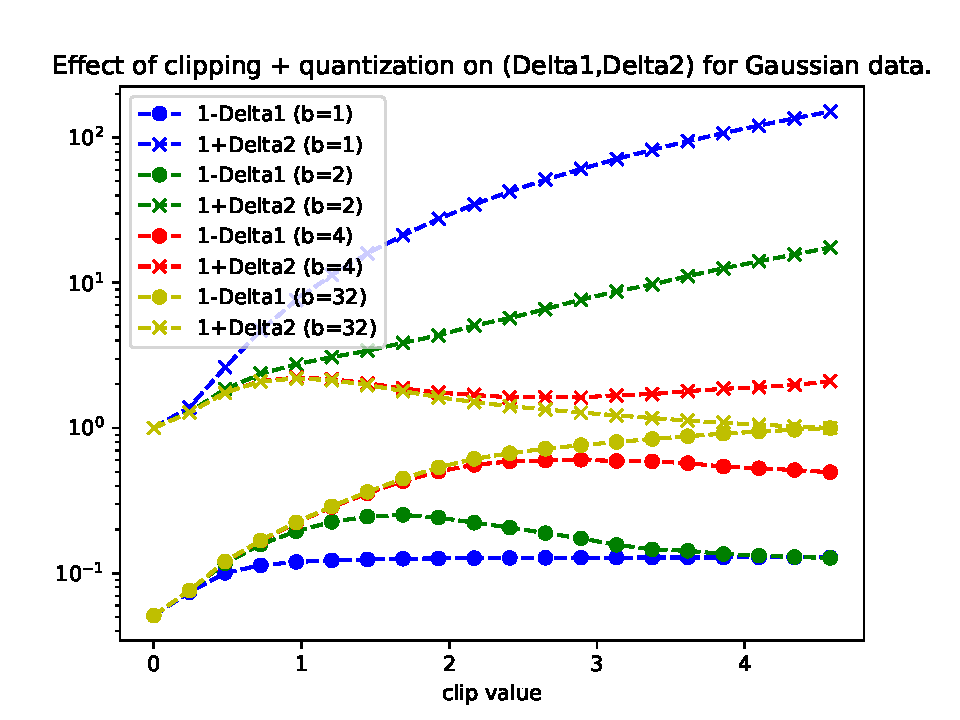
\includegraphics[width=0.8\columnwidth]{figures/deltas_vs_clip_and_quant.pdf}}
		\caption{On random Gaussian data $X \in \RR^{1000\times 30}$, we demonstrate the joint effect of clipping and quantizing on $\Delta_1$ and $\Delta_2$, where we take $\lambda = \sigma_{min}(X^T X)/10$.
		A large clipping value gives large $\Delta_2$, whereas a small clipping values gives large $\Delta_1$.
		This reveals the importance of choosing a clipping value which balances these two considerations.
		}
		\label{fig:deltas_vs_clip_quant}
	\end{center}
\end{figure}
